\documentclass{standalone}

\usepackage{graphics}
\usepackage[dvipsnames,svgnames]{xcolor}

\usepackage{tikz,pgf,pgfplots,circuitikz}
\pgfplotsset{compat=1.15}
\usetikzlibrary{shapes.symbols,intersections,arrows.meta,angles,calc,3d,decorations.pathmorphing}
\usepackage[compat=1.1.0]{tikz-feynhand}

\usepackage{amssymb,amsfonts,amsthm,mathtools}
\usepackage{physics,braket,bm}

\begin{document}

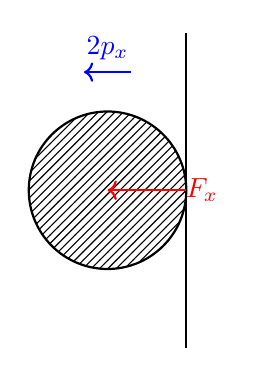
\begin{tikzpicture}
  % Draw the vertical line
  \draw[thick] (3, 0) -- (3, 4);

  % Draw the circle with hatching
  \draw[thick] (2, 2) circle (1);
  \fill[pattern=north east lines] (2, 2) circle (1);

  % Draw the horizontal red arrow inside the circle
  \draw[thick, red, ->] (3,2) -- (2, 2);
  \node[red] at (3.2, 2) {$F_x$};

  % Draw the blue arrow on the left
  \draw[thick, blue, ->] (2.3, 3.5) -- (1.7, 3.5);
  \node[blue] at (2, 3.8) {$2p_{x}$};
\end{tikzpicture}

\end{document}
